%!TEX root = bambi-thesis.tex

\chapter{MAVLink Protocol} % (fold)
\label{appendix:mavlink}
\textit{“MAVLink is a very lightweight messaging protocol for communicating with drones (and between onboard drone components).\\
MAVLink follows a modern hybrid publish-subscribe and point-to-point design pattern: Data streams are sent / published as topics while configuration sub-protocols such as the mission protocol or parameter protocol are point-to-point with retransmission.\\
Messages are defined within XML files. Each XML file defines the message set supported by a particular MAVLink system, also referred to as a "dialect". The reference message set that is implemented by most ground control stations and autopilots is defined in common.xml (most dialects build on top of this definition).\\
The MAVLink toolchain uses the XML message definitions to generate MAVLink libraries for each of the supported programming languages. Drones, ground control stations, and other MAVLink systems use the generated libraries to communicate. These are typically MIT-licensed, and can therefore be used without limits in any closed-source application without publishing the source code of the closed-source application.”} \cite{Mavlink}
\paragraph{Key Features} % (fold)
\label{par:key_features}
\begin{itemize}
	\item Very efficient. MAVLink 1 has just 8 bytes overhead per packet, including start sign and packet drop detection. MAVLink 2 has just 14 bytes of overhead (but is a much more secure and extensible protocol). Because MAVLink doesn't require any additional framing it is very well suited for applications with very limited communication bandwidth. 
	\item Very reliable. MAVLink has been used since 2009 to communicate between many different vehicles, ground stations (and other nodes) over varied and challenging communication channels (high latency/noise). It provides methods for detecting packet drops, corruption, and for packet authentication.
	\item Supports many programming languages, running on numerous microcontrollers/operating systems (including ARM7, ATMega, dsPic, STM32 and Windows, Linux, MacOS, Android and iOS).
	\item Allows up to 255 concurrent systems on the network (vehicles, ground stations, etc.)
	\item Enables both offboard and onboard communications (e.g. between a GCS and drone, and between drone autopilot and MAVLink enabled drone camera). 
\end{itemize}


% paragraph key_features (end)

% \begin{figure}[ht]
%     \centering
%     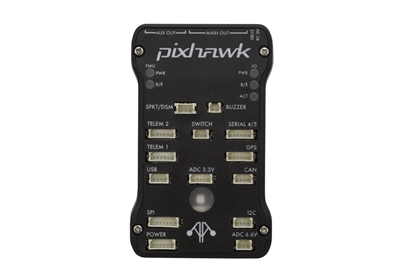
\includegraphics[width=.6\textwidth]{figures/A1/pixhawk.jpg}
%     \caption{}
%     \label{fig:Pixhawk Flight Controller}
% \end{figure}
